\chapter{Adaptive Optics Control Software}
\label{chpt:ao_tools}

Implementing adaptive optics (AO) in microscopy has already been shown to be highly effective at removing optical aberrations and yielding significantly improvements to image quality.\cite{booth2014adaptive,girkin2009adaptive} However, AO technology has not been widely adopted due to a number of barriers. Firstly, it is not trivial to set-up an AO element such as the deformable mirrors (DMs) present in the Aurox Clarity system and DeepSIM optical paths. The DM must be calibrated to meaningfully recreate and correct aberrations. Performing this callibration step is not something non-specialist user may know how to do, or how to assess if the process has been successful. Secondly, measuring the wavefront deformations (and therefore the aberrations) present in a sample is complicated. While techniques to directly measure the  wavefront do exits, they carry additional complications and are only applicable in certain samples.\cite{wang2014rapid,wang2015direct} Therefore indirect wavefront sensing is generally preferred which requires inferring the aberrations present from the variance of a measure of the image quality.\cite{rodriguez2018adaptive} This adds an additional complication since there is no universal image quality metric. Indeed, the best metric often varies with sample type and imaging modality.\cite{burke2015adaptive,booth2002adaptive,fienup2003aberration,debarre2008adaptive} So far, a robust, easy-to-use implementation which incorporates multiple AO methods for multiple sample types/imaging modalities has yet to be presented.\cite{ji2017adaptive}

Microscope-AOtools provides such an implementation, utilising Python-Microscope to control the physical hardware. It incorporates methods for calibrating a DM, evaluating the success of the calibration in recreating aberrations and performing both direct wavefront sensing and sensorless adaptive optics corrections. The methods for sensorless adaptive optics correction can utilise a number from a suite of image quality metrics that can be easily extended to include additional sample or imaging method-specific metrics. These methods are automated, require minimal user involvement and setup and are tied to simple, descriptive  buttons on the Cockpit UI allowing for greater accessibility to users, shown in Figure~\ref{fig:DeepSIM_control_software}. The functions specific to the DM are shown in Figure~\ref{fig:DM_methods_cockpit}. These methods are divided into two categories; Set-up methods and Sample Correction methods. Figures~\ref{fig:DM_methods_cockpit_options} -~\ref{fig:DM_sensorless_ao_parameters} are optional windows that can be used by advanced users to change certain parameters used in the correction routines. How these parameters affect the correction routines will be explained in the relevant sections.

\begin{figure}[H]
	\centering
	\begin{subfigure}{0.25\textwidth}
		\centering
		\includegraphics[width=\linewidth]{images/DM_methods_cockpit.jpg}
		\caption{}
		\label{fig:DM_methods_cockpit}
	\end{subfigure}
	\begin{subfigure}{0.5\textwidth}
		\centering
		\includegraphics[width=\linewidth]{images/DM_methods_cockpit_options.png}
		\caption{}
		\label{fig:DM_methods_cockpit_options}
	\end{subfigure}
	
	\begin{subfigure}{0.45\textwidth}
		\centering
		\includegraphics[width=\linewidth]{images/direct_wavefront_sensing_options.jpg}
		\caption{}
		\label{fig:DM_direct_wavefront_sensing_options}
	\end{subfigure}
	\begin{subfigure}{0.35\textwidth}
		\centering
		\includegraphics[width=\linewidth]{images/sensorless_ao_parameters.jpg}
		\caption{}
		\label{fig:DM_sensorless_ao_parameters}
	\end{subfigure}
	\caption[Cockpit GUI DM specific functionality]{Cockpit GUI DM specific functionality. \textbf{(a)} Deformable mirror specific functions on the Cockpit UI \textbf{(b)} Options window used for changing the image quality metric used in the sensorless AO routine and to spawn additional parameter varying windows. Spawned by right-clicking on the AO methods \textbf{(c)} Options window for varying the parameters used in the system aberration routing correction routing. Spawned by the "Set System Flat Calculation Parameters" button \textbf{(d)} Options window for varying the parameters used in the sensorless AO routine. Spawned by the "Set Sensorless Parameters" button}
	\label{fig:DeepSIM_control_software}
\end{figure}

\section{Set-up Methods}
\label{sec:set_up_methods}

As previously described, DeepSIM has multiple beam paths; interferometric, widefield and SIM. The interferometric beam path is used for calibrating the deformable mirror. An image is formed by the interference between the reference beam arm and the system beam arm. The size of the reference beam is larger than that of the system beam to ensure easy alignment between the two arms. It is therefore necessary to have a method for selecting the interferometric region of interest (ROI) i.e. the region where the reference and system beam arms interfere. Cockpit implements such a method as the functionality of the "Select ROI" button shown in Figure~\ref{fig:DM_methods_cockpit}. This spawns the window shown in Figure~\ref{fig:ROI_selectors} where the user can draw a circle which will define the interferometric ROI. This coordinates of this ROI are saved to the microscope's configuration files with the "Save ROI" button.

\begin{figure}[h]
	\centering
	\begin{subfigure}{0.4\textwidth}
		\centering
		\includegraphics[width=1\linewidth]{images/ROI_selector_init.jpg}
		\caption{}
		\label{fig:ROI_selector_init}
	\end{subfigure}
	\begin{subfigure}{0.4\textwidth}
		\centering
		\includegraphics[width=1\linewidth]{images/ROI_selector.jpg}
		\caption{}
		\label{fig:ROI_selector}
	\end{subfigure}
	\caption[User interface for selecting the interferometric region of interest]{User interface for selecting the interferometric region of interest \textbf{(a)} The ROI selecter UI when it is first initialised \textbf{(b)} UI with the ROI selected}
	\label{fig:ROI_selectors}
\end{figure}

\subsection{Direct wavefront sensing}
\label{subsec:direct_wavefront_sensing}

The two most common methods for direct wavefront sensing are Shack-Hartmann and interferometric methods. Shack-Hartmann wavefront sensing is useful for instances where accuracy is less important than the speed of wavefront recovery. While these situations do exist, the current use-cases for direct wavefront sensing within DeepSIM and Microscope-AOtools are calibration and system aberration correction. These are both situation where accuracy is considerably more important than speed. Additionally, implementing phase extraction from interferometric data has proven more challenging  to automate than from Shack-Hartmann sensor data. Interferometric data can be defined as:

\begin{equation}\label{eq:I_basic}
I(x,y,t) = a(x,y) + b(x,y)cos[\phi(x,y) + \Phi_{R}(x,y,t)]
\end{equation}

Where $a(x,y)$ describes the variation of the background illumination, $b(x,y)$ describes the noise and contrast variations, $\phi(x,y)$ describes the phase imparted by the DM surface and $\Phi_{R}(x,y,t)$ is the reference phase at time $t$. $\Phi_{R}(x,y,t)$ is an offset in the measured phase position, and any variation in this term shifts the lateral position of the entire interference pattern. The relevant phase information is encoded in the $\phi(x,y)$ term and this term specifies shape and spacing of the interference pattern. $\Phi_{R}(x,y,t)$ can therefore be arbitrarily set to 0, simplifying the cosine term in Equation~\ref{eq:I_basic} to $cos[\phi(x,y)]$. Expanding this simplified cosine term using Euler's formula, as well as the definition that $c(x,y) = \frac{1}{2}b(x,y)e^{i\phi(x,y)}$, leads to:

\begin{equation}\label{eq:I_cos_expand}
I(x,y) = a(x,y) + c(x,y) + c^{*}(x,y)
\end{equation}

Where $c^{*}(x,y)$ is the complex conjugate of $c^{*}(x,y)$. Applying the 2-D Fourier transform Equation~\ref{eq:I_cos_expand} becomes:

\begin{equation}\label{eq:I_fourier}
\boldsymbol{I}(u,v) = \boldsymbol{A}(u,v) + \boldsymbol{C}(u,v) + \boldsymbol{C}^{*}(u,v)
\end{equation}

Where, $\boldsymbol{I}(u,v)$, $\boldsymbol{A}(u,v)$, $\boldsymbol{C}(u,v)$ and  $\boldsymbol{C}^{*}(u,v)$ are the Fourier transforms of $I(u,v)$, $a(u,v)$, $c(u,v)$ and $c^{*}(u,v)$ respectively. Now, given that $I(x,y)$ is real valued, it naturally follows that $\boldsymbol{I}(u,v)$ is Hermitian. The amplitude spectrum is symmetric around the zero position (i.e. $u = 0$, $v = 0$). It follows then that $\boldsymbol{C}(u,v)$ and $\boldsymbol{C}^{*}(u,v)$ must contain the same information, only centred on different spatial frequencies. One can apply a bandpass filter in the spatial frequency domain to remove both $\boldsymbol{A}(u,v)$ and $\boldsymbol{C}^{*}(u,v)$ to leave only $\boldsymbol{C}(u,v)$.\cite{lewis1993absolute} Applying the inverse Fourier transform yields $c(x,y)$, which is now complex. The phase of the wavefront can then be recovered by:

\begin{equation}\label{eq:phase}
\phi(x,y) = \arctan\left(\frac{\Im\{c(x,y)\}}{\Re\{c(x,y)\}}\right)
\end{equation}

In the phase acquisition workflow shown in Figure~\ref{fig:phase_unwrap_workflow}, these mathematical steps are implemented in a practical way. The interferogram (\ref{fig:puw_inteferogram}) is cropped (\ref{fig:puw_inteferogram_cropped}) and the ROI, that is the area described by Equation~\ref{eq:I_basic}, is isolated by masking out all the information outside the ROI. The desired ROI is provided by the user using the ROI selector shown in Figure~\ref{fig:ROI_selector}. Quadrant shifting the image (\ref{fig:puw_data_fftshift}) and applying a tukey window mask (\ref{fig:puw_tukey_window}) is done to minimise the spurious spatial frequencies which arise from performing a fast Fourier transform (FFT) on an image with sharp discontinuities at the quadrant edges.

\begin{figure*}
	\centering
	\begin{subfigure}{0.23\textwidth}
		\centering
		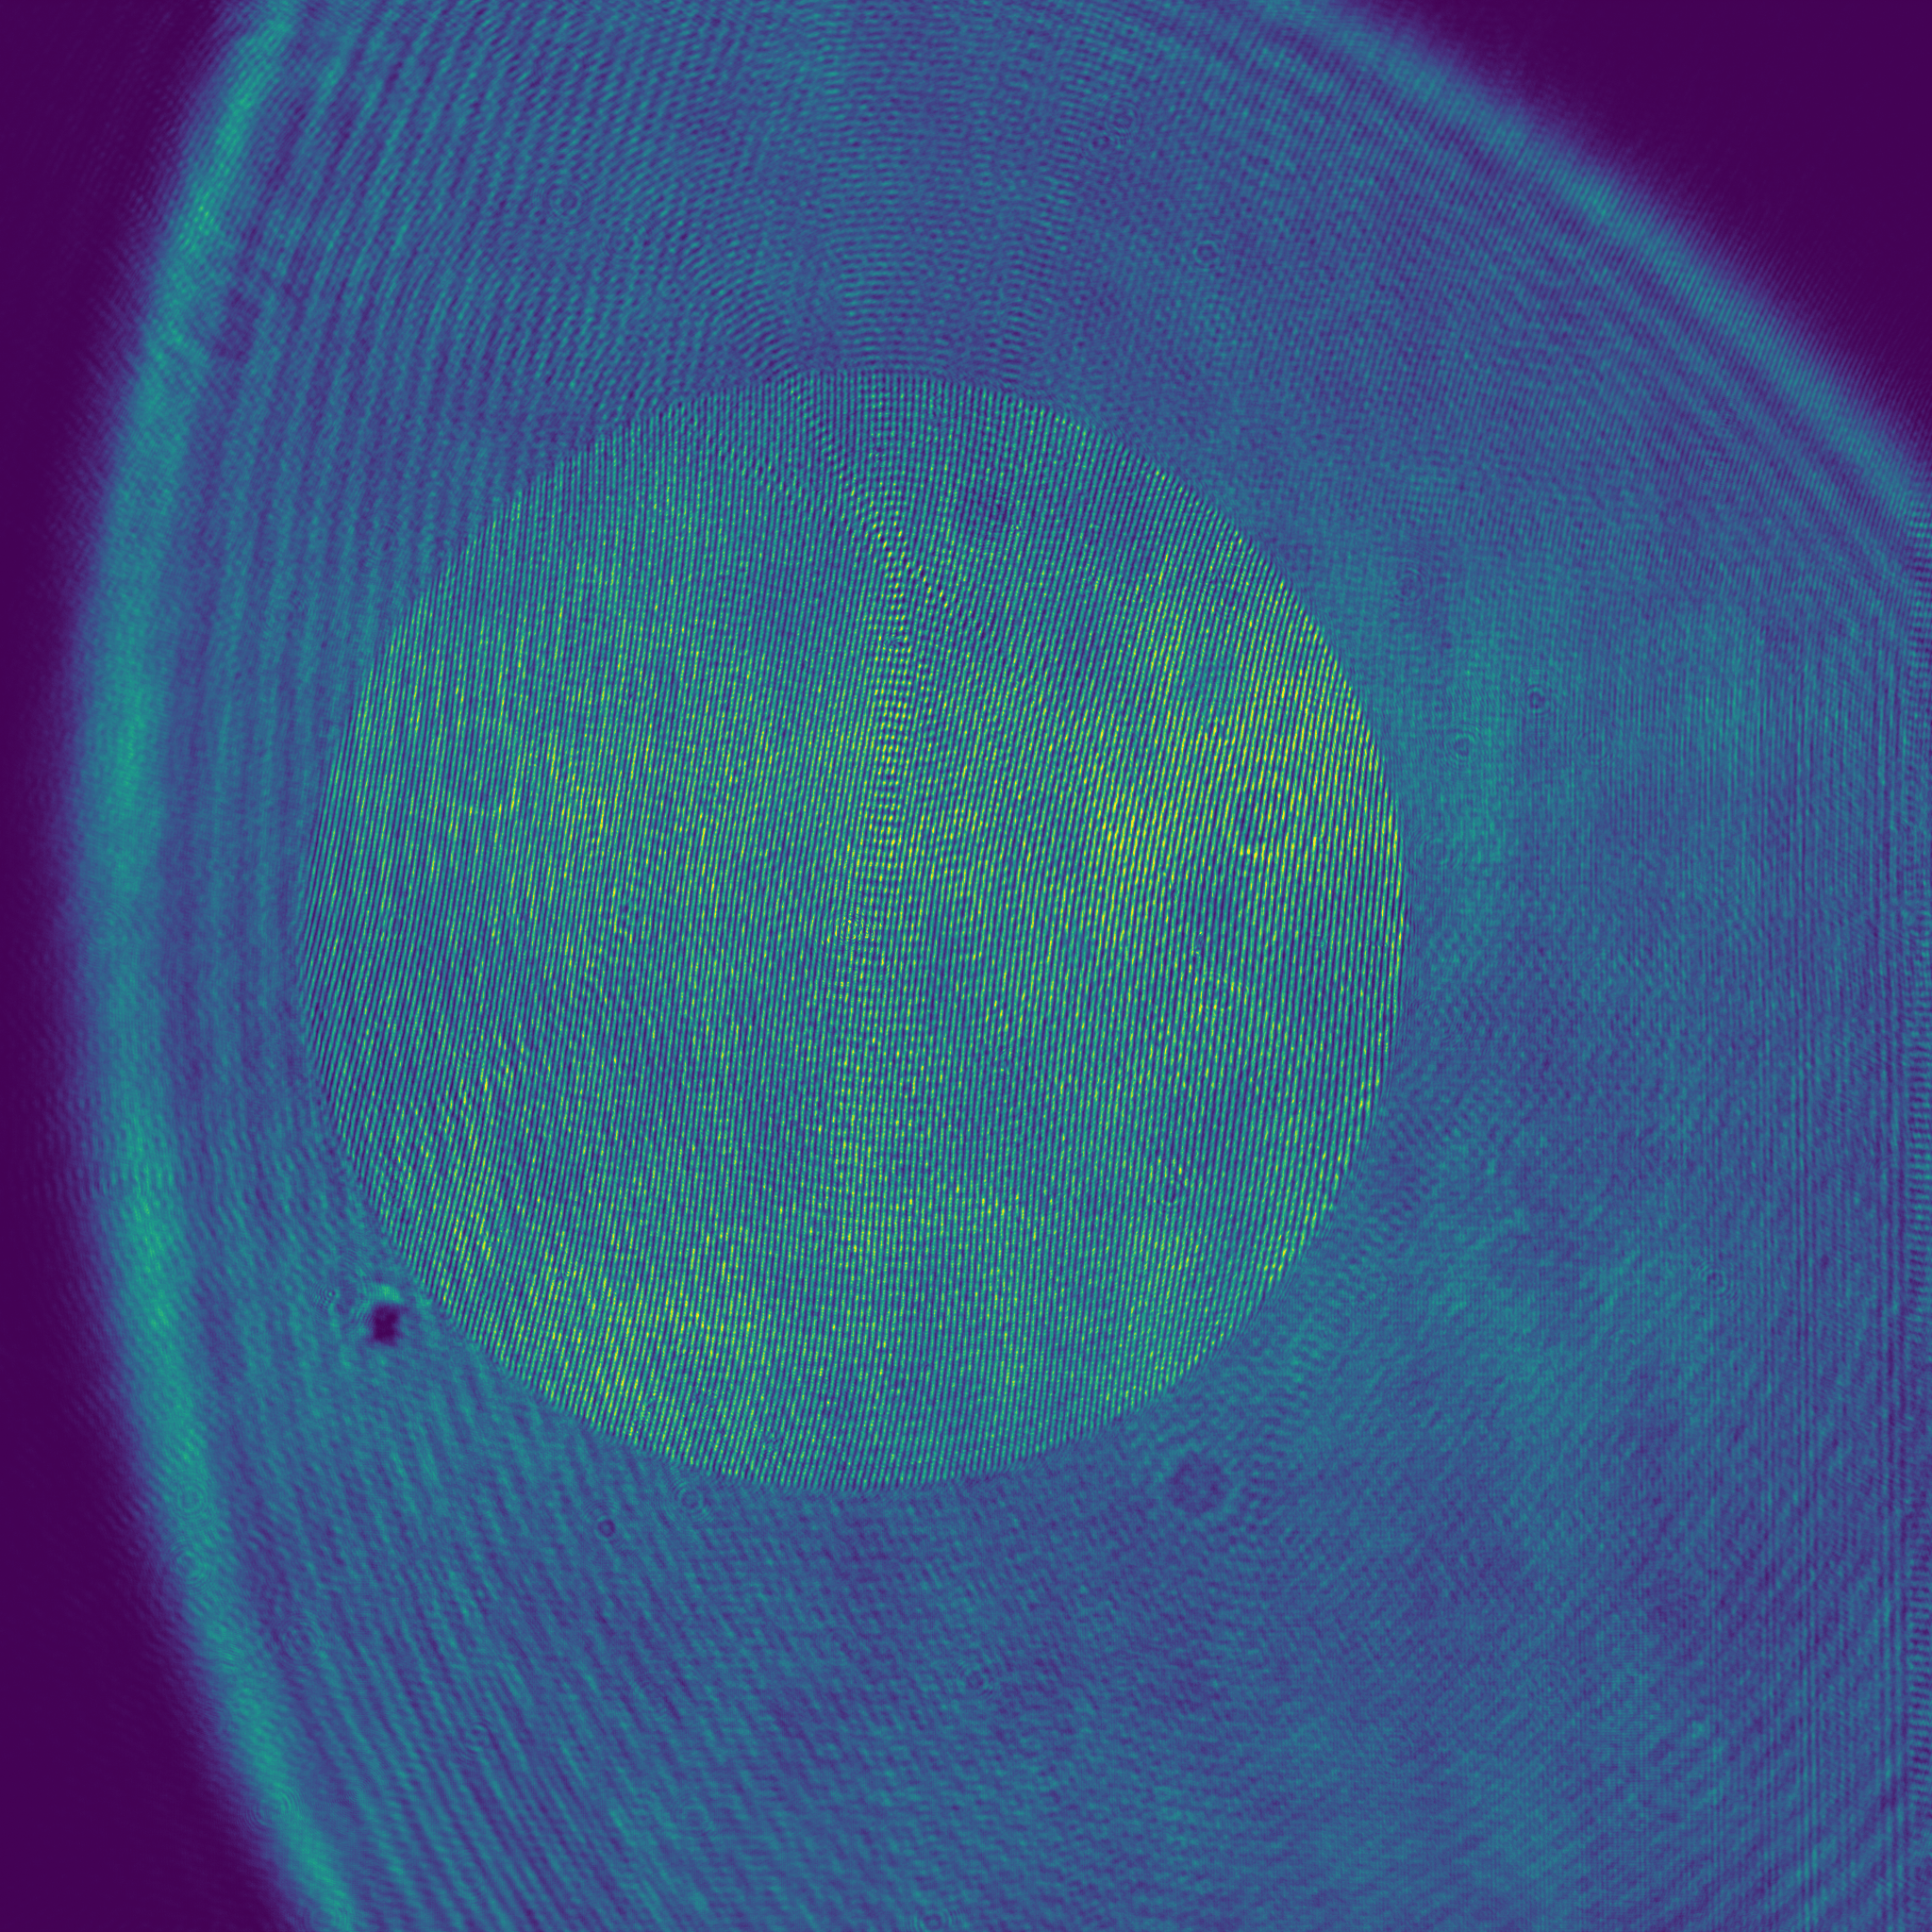
\includegraphics[width=1\linewidth, scale=0.5]{images/puw_inteferogram.png}
		\caption{}
		\label{fig:puw_inteferogram}
	\end{subfigure}
	\begin{subfigure}{0.23\textwidth}
		\centering
		\includegraphics[width=1\linewidth, scale=0.5]{images/puw_inteferogram_cropped.png}
		\caption{}
		\label{fig:puw_inteferogram_cropped}
	\end{subfigure}
	\begin{subfigure}{0.23\textwidth}
		\centering
		\includegraphics[width=1\linewidth, scale=0.5]{images/puw_mask.png}
		\caption{}
		\label{fig:puw_mask}
	\end{subfigure}
	\begin{subfigure}{0.23\textwidth}
		\centering
		\includegraphics[width=1\linewidth, scale=0.5]{images/puw_data_masked.png}
		\caption{}
		\label{fig:puw_data_masked}
	\end{subfigure}
	
	\begin{subfigure}{0.23\textwidth}
		\centering
		\includegraphics[width=1\linewidth, scale=0.5]{images/puw_data_fftshift.png}
		\caption{}
		\label{fig:puw_data_fftshift}
	\end{subfigure}
	\begin{subfigure}{0.23\textwidth}
		\centering
		\includegraphics[width=1\linewidth, scale=0.5]{images/puw_tukey_window.png}
		\caption{}
		\label{fig:puw_tukey_window}
	\end{subfigure}
	\begin{subfigure}{0.23\textwidth}
		\centering
		\includegraphics[width=1\linewidth, scale=0.5]{images/puw_fringes_tukey.png}
		\caption{}
		\label{fig:puw_fringes_tukey}
	\end{subfigure}
	\begin{subfigure}{0.23\textwidth}
		\centering
		\includegraphics[width=1\linewidth, scale=0.5]{images/puw_new_fringe_fft.png}
		\caption{}
		\label{fig:puw_new_fringe_fft}
	\end{subfigure}
	
	\begin{subfigure}{0.23\textwidth}
		\centering
		\includegraphics[width=1\linewidth, scale=0.5]{images/puw_new_fringe_fft_centre_blocked.png}
		\caption{}
		\label{fig:puw_new_fringe_fft_centre_blocked}
	\end{subfigure}
	\begin{subfigure}{0.23\textwidth}
		\centering
		\includegraphics[width=1\linewidth, scale=0.5]{images/puw_fft_filter.png}
		\caption{}
		\label{fig:puw_fft_filter}
	\end{subfigure}
	\begin{subfigure}{0.23\textwidth}
		\centering
		\includegraphics[width=1\linewidth, scale=0.5]{images/puw_new_fringe_order1.png}
		\caption{}
		\label{fig:puw_new_fringe_order1}
	\end{subfigure}
	\begin{subfigure}{0.23\textwidth}
		\centering
		\includegraphics[width=1\linewidth, scale=0.5]{images/puw_order1_roll.png}
		\caption{}
		\label{fig:puw_order1_roll}
	\end{subfigure}
	
	\begin{subfigure}{0.23\textwidth}
		\centering
		\includegraphics[width=1\linewidth, scale=0.5]{images/puw_complex_phase.png}
		\caption{}
		\label{fig:puw_complex_phase}
	\end{subfigure}
	\begin{subfigure}{0.23\textwidth}
		\centering
		\includegraphics[width=1\linewidth, scale=0.5]{images/puw_phaseorder1.png}
		\caption{}
		\label{fig:puw_phaseorder1}
	\end{subfigure}
	\begin{subfigure}{0.23\textwidth}
		\centering
		\includegraphics[width=1\linewidth, scale=0.5]{images/puw_phaseorder1mask}
		\caption{}
		\label{fig:puw_phaseorder1mask}
	\end{subfigure}
	\begin{subfigure}{0.23\textwidth}
		\centering
		\includegraphics[width=1\linewidth, scale=0.5]{images/puw_unwrapped_phase.png}
		\caption{}
		\label{fig:puw_unwrapped_phase}
	\end{subfigure}
	\caption[Visualisation of the stages of the phase acquisition workflow.]{Visualisation of the stages of the phase acquisition workflow. \textbf{(a)} Captured interferogram \textbf{(b)} Interferogram cropped to region of interest (ROI) \textbf{(c)} Circular mask \textbf{(d)} ROI isolated \textbf{(e)} ROI quadrant shifted (ROI-qs) \textbf{(f)} 2-D tukey window mask \textbf{(g)} ROI-qs with tukey mask applied \textbf{(h)} Fast Fourier transform (FFT) of \textbf{(g)}, log scaled \textbf{(i)} Fourier transform with the central spatial frequencies masked, log scaled \textbf{(j)} 2-D sine squared mask centred on the position of spatial frequencies encoding the phase information \textbf{(k)} The original Fourier transform, \textbf{(h)}, with the sine squared mask applied \textbf{(l)} Phase encoding spatial frequencies rolled to the central position \textbf{(m)} Inverse FFT of the phase encoding spatial frequencies \textbf{(n)} Inverse FFT transformed into a phase map \textbf{(o)} Phase map masked to isolate ROI \textbf{(p)} Phase map unwrapped to remove 2$\pi$ discontinuities}
	\label{fig:phase_unwrap_workflow}
\end{figure*}

Having performed the FFT (\ref{fig:puw_new_fringe_fft}), an array described by Equation~\ref{eq:I_fourier} is obtained. A selection of the central spatial frequencies are masked (\ref{fig:puw_new_fringe_fft_centre_blocked}), primarily to mask out the central spatial frequency which represents the mean intensity and has an amplitude orders of magnitude larger than any other spatial frequency. The spatial frequencies which now have the highest amplitudes correspond to both $\boldsymbol{C}(u,v)$ and $\boldsymbol{C}^{*}(u,v)$. One of the aforementioned amplitude peaks is located and a bandpass filter described by $\sin^{2}(x,y)$ is constructed (\ref{fig:puw_fft_filter}) centred on the spatial frequency location of this amplitude peak. As previously noted, the Fourier transform of the interferogram is symmetrical around the central spatial frequency. So, it doesn't matter which of the two peaks this filter is centred on since they encode the same information. The aforementioned bandpass filter is then applied to the FFT of the interferogram (\ref{fig:puw_new_fringe_order1}) and these spatial frequencies are then rolled to the central spatial frequency position (\ref{fig:puw_order1_roll}). Applying this successfully filters $\boldsymbol{A}(u,v)$ and $\boldsymbol{C}^{*}(u,v)$, isolating $\boldsymbol{C}(u,v)$ as desired.

The array corresponding to $\boldsymbol{C}(u,v)$ is inverse Fourier transformed to yield $c(x,y)$ (\ref{fig:puw_complex_phase}). This is then converted to a phase map by performing the calculation in Equation~\ref{eq:phase} (\ref{fig:puw_phaseorder1}) and the mask in Figure~\ref{fig:puw_mask} is applied again to mask out any spurious noise outside the ROI. Due to the periodic nature of trigonometric functions, this phase map is wrapped around $-\pi$ and $\pi$. An 2D  algorithm is used to unwrap the phase map and yield a phase Figure~\ref{fig:puw_unwrapped_phase} is obtained.\cite{herraez2002fast} Other than determining the appropriate ROI, this workflow is entirely automated and requires no user input. 

Automation does have a drawback. The location of the phase component of the Fourier transform is determined by finding the maximum intensity in the data represented by Figure~\ref{fig:puw_new_fringe_fft_centre_blocked} and then performing a number of centre of mass calculations to find the `true' centre of the phase component. However, this `true' centre may still be incorrect by a few pixels. This offset leads to an artificial introduction of tip and/or tilt in the final wavefront and this artificial tip/tilt cannot be separated from the true tip/tilt. Therefore, the described phase acquisition implementation cannot be said to be sensitive to tip or tilt. However, since tip and tilt (along with piston) are not considered to be a true optical aberration, this is a small price to pay for a fully automated phase acquisition workflow.

This phase extraction technique is used as part of other methods, but it is also useful for a user to be able to visualise the wavefront phase map. Principally this is because if the interferogram is not well focused on the camera it can result in the wavefront being heavily distorted by the Zernike mode corresponding to the defocus optical aberration (Noll Index 4). This can mask smaller wavefront deformations caused by the movement of the DM actuators and therefore bias calibration measurements. It can also be useful to view the system aberrations present, to check the difference applying the system aberration correction makes to the wavefront shape and to manually check for discontinuities. Cockpit implements such a method as the functionality of the "Visualise Phase" button shown in Figure~\ref{fig:DM_methods_cockpit}. This spawns the window shown in Figure~\ref{fig:phase_viewer_phase}, displaying the phase wavefront acquired from the interferogram. The display can be changed to the power spectrum of the interferogram, Figure~\ref{fig:phase_viewer_ft}, and back by pressing the "Real/Fourier Transform switch" button. 

\begin{figure}[h]
	\centering
	\begin{subfigure}{0.45\textwidth}
		\centering
		\includegraphics[width=1\linewidth, scale=0.5]{images/phase_viewer_phase.jpg}
		\caption{}
		\label{fig:phase_viewer_phase}
	\end{subfigure}
	\begin{subfigure}{0.45\textwidth}
		\centering
		\includegraphics[width=1\linewidth, scale=0.5]{images/phase_viewer_ft.jpg}
		\caption{}
		\label{fig:phase_viewer_ft}
	\end{subfigure}
	\caption[User interface for viewing the phase wavefront]{User interface for viewing the phase wavefront \textbf{(a)} Phase viewer window showing the unwrapped phase acquired from the interferogram \textbf{(b)} Phase viewer window showing the power spectrum of the interferogram. }
	\label{fig:phase_viewer}
\end{figure}

\subsection{Calibration}
\label{subsec:calibration}

For aberration correction, one could attempt to measure the overall aberration of the optical wavefront and apply the opposite shape to the DM. For direct wavefront sensing, this would appear as simple as measuring the phase distortion and shaping the DM to cancel this distortion. However, for continuous membrane DMs (which the majority of commercially available DMs are) the response of mirror shape to the actuators which control the mirror shape is generally non-linear, due to the membrane's mechanical elasticity, electrostatic forces and the coupling between actuators.\cite{Zhu:99} For indirect wavefront sensing this presents an even greater problem since any minimisation of the wavefront aberration would involve \textit{N} degrees of freedom, where \textit{N} is the number of actuators. Assuming that the overall mirror shape is the linear 
superposition of all the individual actuator deflections, we can 
define the overall mirror shape, $S(x,y)$ as:

\begin{equation}\label{eq:surface_shape}
S(x,y) = \sum_{h=1}^{N} d_{h}\phi_{h}(x,y)
\end{equation}

Where $S(x,y)$ is the change in the deformable mirror shape from its original position, $d_h$ is the $h$-th actuator control signal (an arbitrary value related to applied voltage which determines the position the $h$-th actuator in its overall movement range) and $\phi_{h}(x,y)$ is the $h$-th influence function. These are called the influence functions of the AO device since they describe how the elements of the device influence the phase wavefront. We can change this set of basis functions for a different basis set. An obvious alternative basis set is the Zernike polynomials since they are defined on the unit circle, orthogonal and the wavefront distortion can be well approximated by the linear addition of Zernike polynomials\cite{von1934beugungstheorie,noll1976zernike,mahajan1994zernike}. Describing $\phi_{h}(x,y)$ in terms of Zernike polynomials we obtain:

\begin{equation}\label{eq:influence_to_zernike}
\phi_{h}(x,y) = \sum_{g=1}^{M} b_{g,h}z_{g}(x,y)
\end{equation}

Where $b_{g,h}$ is the coefficient corresponding to the $k$-th Zernike polynomial due to the $d_h$. The change in mirror shape, $\Delta S(x,y)$, can therefore be described as:

\begin{equation}\label{eq:zernike_sub}
\begin{split}
\Delta S(x,y) & = \sum_{h=1}^{N} d_{h}\left[\sum_{g=1}^{M} b_{g,h}z_{g}(x,y)\right] \\
& =\sum_{g=1}^{M} \left(\sum_{h=1}^{N} d_{h} b_{g,h}\right) z_{g}(x,y) \\
& =\sum_{g=1}^{M} a_{g} z_{g}(x,y)
\end{split}
\end{equation}

Where the new Zernike coefficients, $a_{g}$, is defined as:

\begin{equation}\label{eq:new_z_coef}
a_{g} = \sum_{h=1}^{N} b_{g,h} d_{h} \text{~for~} g=1,2,...,M
\end{equation}

Converting Equation~\ref{eq:new_z_coef} to a matrix form yields:

\begin{equation}\label{eq:CM_derivation}
\begin{split}
\bar{a} &= \boldsymbol{B} \bar{d}\\
\Rightarrow \bar{d} &= \boldsymbol{C} \bar{a}
\end{split}
\end{equation}

Where $\bar{d}$ is a length $N$ vector of the actuator control signals, $\bar{a}$ is the length $M$ vector of the Zernike polynomial amplitudes and $\boldsymbol{B}$ is the $M \times N$ matrix representing the response characteristics of the deformable mirror. However, we actually want its inverse, $\boldsymbol{B}^{-1} =\boldsymbol{C}$, otherwise called the control matrix in order to convert from Zernike polynomial amplitudes to actuator control signals.

Microscope-AOtools implements an automated calibration routine to obtain $\boldsymbol{C}$. Each actuator is moved through $p$ set positions and a wavefront is extracted. Figure~\ref{fig:observed_wavefront} shows an observed wavefront during the calibration routine. The wavefront is then decomposed into $M$ Zernike modes\cite{townson2019aotools}. A row vector $\boldsymbol{z}$ is obtained for each actuator position containing the computed Zernike mode amplitudes:

\begin{equation}\label{eq:zernike_amp}
\boldsymbol{z} = 
\begin{bmatrix}
z_{1} & z_{2} & \cdots & z_{m} 
\end{bmatrix}
\end{equation}

Where the $g$-th element is the amplitude of the $g$-th
Zernike mode. Figure~\ref{fig:measured_zernike_modes} shows
a plot of the row vector containing the amplitudes of the 
$M$ Zernike modes measured for Figure~\ref{fig:observed_wavefront}.
Figure~\ref{fig:simulated_wavefront} show a simulated wavefront 
constructed using these Zernike mode amplitudes. As previously 
mentioned, a phase wavefront can be constructed from an 
infinite linear combination of Zernike modes\cite{noll1976zernike}. 
However, using a finite number of Zernike modes produces only an 
approximation of the original wavefront. 
Figure~\ref{fig:observed_simulated_wavefront_diff} show the
difference between the two and a ``ringing'' analogous to the 
Gibbs phenomena for recreating periodic signals using a
truncated Fourier series is present.

By collecting the row vectors of each position
for the $h$-th actuator we can obtain:

\begin{equation}\label{eq:zernike_amp_actuator}
A_h = 
\begin{bmatrix}
\boldsymbol{z_{1}}\\
\boldsymbol{z_{2}}\\
\vdots\\
\boldsymbol{z_{p}} 
\end{bmatrix}
=
\begin{bmatrix}
z_{1,1} & z_{1,2} & \cdots & z_{1,m} \\
z_{2,1} & z_{2,2} & \cdots & z_{2,m} \\
\vdots  & \vdots  & \ddots & \vdots  \\
z_{p,1} & z_{p,2} & \cdots & z_{p,m} 
\end{bmatrix}
\end{equation}

Linear regression to each column, $\begin{bmatrix} z_{1,i} & z_{2,i} & \cdots & z_{p,i} \end{bmatrix}^T$, yields the response characteristics between the $h$-th actuator's position and the $g$-th Zernike mode, $b_{g,h}$. Figure~\ref{fig:influence_function_11} shows the influence function fitting for Zernike mode 11 (Noll index) for the $26^{th}$ actuator. The gradient of the slope is, in this case, $b_{11,26}$. This gradient is acquired for each actuator, for each Zernike mode. In this way, we construct $\boldsymbol{B}$ and then calculate $\boldsymbol{C}$. Figure~\ref{fig:calibration_workflow} shows a flowchart of this process as implemented in Microscope-AOtools.

\begin{figure}[h]
	\centering
	\begin{subfigure}{0.285\textwidth}
		\centering
		\includegraphics[width=1\linewidth, scale=0.5]{images/observed_wavefront.png}
		%\caption{Observed wavefront}
		\caption{}
		\label{fig:observed_wavefront}
	\end{subfigure}
	\begin{subfigure}{0.285\textwidth}
		\centering
		\includegraphics[width=1\linewidth, scale=0.5]{images/simulated_wavefront.png}
		%\caption{Simulated wavefront}
		\caption{}
		\label{fig:simulated_wavefront}
	\end{subfigure}
	\begin{subfigure}{0.345\textwidth}
		\vspace{-0.2cm}
		\centering
		\includegraphics[width=1\linewidth, scale=0.5]{images/observed_simulated_wavefront_diff.png}
		%\caption{Difference between observed and simulated wavefront}
		\caption{}
		\label{fig:observed_simulated_wavefront_diff}
	\end{subfigure}
	
	\begin{subfigure}{0.45\textwidth}
		\centering
		\includegraphics[width=1\linewidth, scale=0.5]{images/measured_zernike_modes.png}
		%\caption{Zernike mode amplitudes measured in the observed wavefront}
		\caption{}
		\label{fig:measured_zernike_modes}
	\end{subfigure}
	\begin{subfigure}{0.45\textwidth}
		\centering
		\includegraphics[width=1\linewidth, scale=0.5]{images/influence_function_11.png}
		%\caption{Influence function fitting}
		\caption{}		
		\label{fig:influence_function_11}
	\end{subfigure}
	\caption[Visualisation of the influence function fitting stage of the calibration routine]{Visualisation of the influence function fitting stage of the calibration routine \textbf{(a)} An example observed wavefront obtained during the calibration process for an Alpao-69 actuator deformable mirror. The $26^{th}$ actuator is at the first of the 5 positions. \textbf{(b)} A simulated wavefront created from the 69 Zernike mode amplitudes measured in the observed wavefront. \textbf{(c)} The difference in the observed and simulated wavefronts. \textbf{(d)} The 69 Zernike mode amplitudes measured for the observed wavefront \textbf{(e)} The influence function fitting for Zernike mode 11 (Noll index) for the $26^{th}$ actuator}
	\label{fig:wavefront_decomposition}
\end{figure}

\begin{figure}[h]
	\centering
	\begin{subfigure}{0.45\textwidth}
		\centering
		\includegraphics[width=1\linewidth, scale=0.5]{images/calibration_routine_workflow.jpg}
		\caption{}
		\label{fig:calibration_routine_workflow}
	\end{subfigure}
	\begin{subfigure}{0.45\textwidth}
		\centering
		\includegraphics[width=1\linewidth, scale=0.5]{images/Ith_actuator_calibration_workflow_blue_border.jpg}
		\caption{}
		\label{fig:Ith_actuator_calibration_workflow_blue_border}
	\end{subfigure}
	\caption[Calibration routine workflow]{\textbf{(a)} Flowchart depicting the generalised calibration routine implemented in Mircoscope-AOtools \textbf{(b)} Flowchart depicting the the process for calibrating the $h$-th actuator of the deformable mirror, the dashed blue process in \textbf{(a)}. The influence functions returned are $b_{g,h}$ described in Equation~\ref{eq:influence_to_zernike}. This process is performed for each $N$ actuators and used to obtain $\boldsymbol{C}$ described in Equation~\ref{eq:CM_derivation}.}
	\label{fig:calibration_workflow}
\end{figure}

In general, $\boldsymbol{B}$ is singular and therefore has no true inverse and so we must use a pseudo-inverse, calculated using single value decomposition (SVD). However, some values of $\boldsymbol{B}$ may be small since the physical position of certain actuators will mean they have limited influence on creating certain Zernike modes. A control matrix calculated without thresholding out these small values will quickly lead to a saturation of the DM actuators (i.e. all actuators at their maximum stroke length) when corrections are calculated.\cite{booth2005methods} Therefore the calibration method incorporates a threshold by default and the exact threshold can be varied by experienced users. The calibration routine is initiated by pressing the "Calibrate" button shown in Figure~\ref{fig:DM_methods_cockpit}.

\subsection{Characterisation}
\label{subsec:characterisation}

Feedback on the quality of the calibration process is essential. Ideally, once the deformable mirror is calibrated we have a linear map which allows known quantities of Zernike modes to be applied exactly. This linear map is never exact in practice due to issues; the fact that some parameters, such as the number of steps used to calibrate each actuator and the threshold used in the SVD pseudo-inversion, are chosen empirically, the approximate nature of the pseudo-inverse, discretisation errors (due to discrete sampling of a continuous functions) in the measuring of Zernike modes. etc It is therefore necessary to have some measure of how well the adaptive element is able to recreate desired Zernike modes. This process is called characterisation. The process involves applying a fixed amplitude of single Zernike modes to the adaptive element, measuring the Zernike modes present and comparing the amplitude to that supposedly applied. An automated implementation of this process is present in Microscope-AOtools with the results returned to the user for interrogation. Figure~\ref{fig:characterisation_workflow} shows a flowchart of this method in Microscope-AOtools. 

\begin{figure}[h]
	\centering
	\includegraphics[width=0.4\textwidth, scale=0.5]{./images/characterisation_workflow.jpg}
	\caption[Characterisation routine workflow]{Flowchart depicting the process for characterising a deformable mirror as implemented in Microscope-AOtools}
	\label{fig:characterisation_workflow}
\end{figure}

In an ideal situation, where the control matrix provided a perfect linear map from Zernike mode amplitudes to the adaptive elements degrees of freedom, a characterisation assay like Figure~\ref{fig:characterisation_assay_ideal} is expected, where only the Zernike mode applied is measured. In practice, the adaptive element is better at recreating particular Zernike modes and some Zernike mode coupling is observed i.e. Zernike modes which were not applied to the adaptive element are measured. This leads to characterisation assays like Figure~\ref{fig:characterisation_assay_real}. Here we present a characterisation assay obtained for an Alpao-69 actuator deformable mirror. We define a recreation accuracy metric, $\alpha_{i}$, for each mode:

\begin{equation}\label{eq:recreation_accuracy}
\begin{split}
\alpha_{i} &= \frac{Z'_{i} - \boldsymbol{RMS}(Z'_{j})}{Z_{i}} \\
&= \frac{Z'_{i} - \sqrt{\frac{1}{N-1}\sum_{j=0,j\ne i}^{N} {Z'_{j}}^{2}}}{Z_{i}}
\end{split}
\end{equation}

Where $Z_{i}$ is the applied Zernike mode amplitude, $Z'_{i}$ and $Z'_{j}$ are the measured Zernike mode amplitudes for the current mode and all other modes respectively and $N$ is the number of Zernike modes being assessed. Figure~\ref{fig:real_characterisation_assay_plot_metric_errorbar} shows a plot of this metric for the characterisation assay in Figure~\ref{fig:characterisation_assay_real}. The errorbars are determined by the standard deviation of $\boldsymbol{RMS}(Z'_{j})$

\begin{figure}[h]
	\centering
	\begin{subfigure}{0.45\textwidth}
		\centering
		\includegraphics[width=0.8\linewidth, scale=0.5]{./images/characterisation_assay_ideal.png}
		\caption{}
		\label{fig:characterisation_assay_ideal}
	\end{subfigure}
	\begin{subfigure}{0.45\textwidth}
		\centering
		\includegraphics[width=1\linewidth, scale=0.5]{./images/characterisation_assay_real.png}
		\caption{}
		\label{fig:characterisation_assay_real}
	\end{subfigure}
	\begin{subfigure}{0.9\textwidth}
		\centering
		\includegraphics[width=0.6\linewidth, scale=0.5]{./images/real_characterisation_assay_plot_metric_errorbar.png}
		\caption{}
		\label{fig:real_characterisation_assay_plot_metric_errorbar}
	\end{subfigure}
	\caption[Example characterisation routine results]{Example characterisation routine results \textbf{(a)} An ideal characterisation assay, measuring the recreation accuracy of 68 Zernike modes with applied amplitude of 1 for each \textbf{(b)} A realistic characterisation assay obtained from a calibrated Alpao-69 actuator deformable mirror, measuring the recreation accuracy of 68 Zernike modes with applied amplitude of 1 for each \textbf{(c)} Plot of the recreation accuracy metric for the real characterisation assay shown in \textbf{(b)}. The threshold (red dashed line) is set at 0.75}
	\label{fig:characterisation_assay_results}
\end{figure}

Clearly not all Zernike modes are recreated equally well and  different modes exhibit varying degrees of mode coupling. As previously mentioned, this arises from mathematical approximations,
computational errors and the physical characteristics of the adaptive element. Microscope-AOtools provides the tools to assess the accuracy of Zernike mode recreation, which can be used to inform which modes should be included in the aberration correction algorithms.

The characterisation routine relies on the same generalised phase acquisition method used in the calibration workflow. Recall that this is a user selected method from a suite of phase acquisition methods. The number of Zernike modes assessed, $N$, is the number of modes that have been measured in the calibration step by default, but this can be varied by the user. Once again this preserves generalisability and allows the characterisation method to be used on any arbitrary adaptive element, calibrated for any number of modes and utilising any desired wavefront sensing technique.

\subsection{System Aberration Correction}
\label{subsec:system_correction}

The applications for aberration correction using direct wavefront sensing have been well documented. The wavefront is measured via interferometry, Shack-Hartmann wavefront sensor, fluorescent guide star, etc and decomposed into Zernike modes. Correction can then be calculated and applied for both system and sample induced aberrations. Microscope-AOtools implements a correction method for situations where the wavefront is directly observed. The workflow is shown in Figure~\ref{fig:direct_wavefront_flattening_workflow}. The wavefront is obtained through whatever direct wavefront sensing method has been implemented and selected, a number of Zernike modes determined by the user are fitted to the wavefront, an equal and opposite magnitude of these modes are applied to the DM. The RMS wavefront error is then calculated. This process repeats until $N$ iterations have been performed or the RMS wavefront error is below a user defined error threshold, $\delta$.

\begin{figure}[h]
	\centering
	\includegraphics[width=0.55\textwidth, scale=0.5]{./images/direct_wavefront_flattening_workflow.jpg}
	\caption[Direct wavefront correction workflow]{Flowchart depicting the process for flattening directly measured wavefront as implemented in Microscope-AOtools}
	\label{fig:direct_wavefront_flattening_workflow}
\end{figure}

In an ideal setup with a perfect control matrix, this process would only need to be performed once. However, as we have already discussed, the control matrices generated for any setup are never ideal due to non-linearities and inter-actuator coupling. Therefore, one iteration of this method would correct the aberrations to an extent, but it would leave residual aberrations. It is necessary to perform this process for a number of iterations to ensure the optimal wavefront is obtained. 

Figure~\ref{fig:direct_wavefront_correction} shows the results of one such wavefront correction, performed using the same Alpao-69 actuator deformable mirror as shown in Figure~\ref{fig:DeepSIM_complete_beam_paths}. The wavefront was 
obtained by interferometry and Zernike modes 5-29 (using Noll indices) were corrected over 20 iterations. The RMS phase errors in Figures~\ref{fig:aberrated_wavefront_defocus_ptt_rmv_crop_phase_only} and \ref{fig:flattened_wavefront_20it} are 3.818 radians and 0.986 radians of 543nm respectively. A significant portion of the phase deformation after correction seems to be located at the edges of the aperture. The RMS phase error of the central 95\% of the phase wavefront is 0.712 radians, equivalent of a Strehl ratio $\approx 0.602$. Figure~\ref{fig:zernike_modes_to_show_flattening}
shows the Zernike mode amplitudes before and after correction. The dots visible are the physical location of the actuators on the deformable mirror and represent a limiting factor in how flat the deformable mirror surface can actually be. 

\begin{figure}[h]
	\centering
	\begin{subfigure}{0.4\textwidth}
		\centering
		\includegraphics[width=1\linewidth, scale=2]{./images/system_wavefront_before_correction_adv.png}
		\caption{}
		\label{fig:aberrated_wavefront_defocus_ptt_rmv_crop_phase_only}
	\end{subfigure}
	\begin{subfigure}{0.49\textwidth}
		\centering
		\vspace{-.25cm}
		\includegraphics[width=1\linewidth, scale=2]{./images/system_wavefront_after_correction_best_20it_adv.png}
		\caption{}
		\label{fig:flattened_wavefront_20it}
	\end{subfigure}
	
	\begin{subfigure}{0.55\textwidth}
		\centering
		\includegraphics[width=1\linewidth, scale=1]{./images/Zernike_modes_before_after_correction_only_corrected.png}
		\caption{}
		\label{fig:zernike_modes_to_show_flattening}
	\end{subfigure}
	\caption[Example direct wavefront correction results]{Example direct wavefront correction results \textbf{(a)} An aberrated wavefront \textbf{(b)} A wavefront after 20 iterations of correction \textbf{(c)} The Zernike mode amplitudes measured in the aberrated (red) and corrected (blue) wavefronts \textbf{(a)} - \textbf{(b)} are all presented on the same colorscale (in radians of 543nm HeNe laser) and were obtains via interferometry}
	\label{fig:direct_wavefront_correction}
\end{figure}

For system aberration corrections it may be preferable to set a minimum wavefront error and continue to iterate until this threshold is reached. However a user may wish to only spend $N$ iterations correcting the wavefront. Microscope-AOtools implements both options to ensure generalisability and these parameters can be set by the user utilising the option window shown in Figure~\ref{fig:DM_direct_wavefront_sensing_options}. As with the calibration and characterisation methods, the wavefront flattening routine relies on a user selected phase acquisition method selected from the suite of implemented phase acquisition methods. This generalised construction ensures that the applicability of Microscope-AOtools to any adaptive element with any wavefront sensing technique is preserved throughout all the set-up methods.

The characterisation routine is initiated by pressing the "Calculate System Flat" button shown in Figure~\ref{fig:DM_methods_cockpit}. Spawning the window shown in Figure~\ref{fig:DM_direct_wavefront_sensing_options} allows a user to vary the number of iterations and RMS error threshold used for the wavefront correction routine. By default the routine runs for exactly 10 iterations, since the default error threshold is $\infty$ and so any wavefront deformation will yield an RMS value under this threshold. A user can also vary the Zernike modes the wavefront flatting routine will try to correct for. By default the Zernike modes corrected for are all Zernike modes with Noll indices, $j$, $\ge$ 4 (i.e. all the true optical aberrations) and $<$ the number of actuators, N. Once the Characterisation routine has been performed this is changed to be all Zernikes modes with $4 \le j < N$ and with a recreation accuracy within 1 standard deviation of 0.75.  Once the actuator values for correcting the system aberrations have been calculated they are stored in Cockpit's internal configuration and can be applied at any time using the "System Flat" button shown in Figure~\ref{fig:DM_methods_cockpit}.

\section{Sample Correction Methods}
\label{sec:sample_correction_methods}

\subsection{Sensorless Correction}
\label{subsec:sensorless_correction}

In many biological applications, direct wavefront sensing is not possible and so we rely on sensorless techniques to determine the best correction to apply. The generalised methodology for this is shown in Figure~\ref{fig:sensorless_correction_method}. Some metric, $S$, which gives a useful measure of the image quality is chosen. This metric should be a numerical value and should 
increase to a global maximum as the aberrations present decrease. Often these metrics are related to common measures of image quality, such as sharpness or contrast. For each Zernike mode, $Z_{i}$, a number of amplitudes of that mode, $a_{j}$, are applied and an image of the sample obtained. The quality of each image, $S_{j}$ is calculated. Assuming that $S$ is a function of the Zernike mode amplitude applied,	fitting a Gaussian function to the $S_{j}$ values yields a Zernike mode amplitude, $a_{max}$, which theoretically yields the best image quality, $S_{max}$. The complexity of sensorless AO correction lies in selecting the most appropriate image quality metric. There 
have been numerous metrics developed which have been shown to be effective on certain sample types or imaging modalities\cite{burke2015adaptive,booth2002adaptive,fienup2003aberration,debarre2008adaptive}.

\begin{figure}[h]
	\centering
	\includegraphics[width=1\textwidth,scale=0.5]{./images/sensorless_aberration_fitting_w_images.png}
	\caption[Principle of sensorless adaptive optics correction.]{Principle of sensorless adaptive optics correction. For each Zernike mode, $Z_i$, images of the sample with different amplitudes of the $i$-th Zernike mode are obtained. A value of the image quality metric, $S$, is obtained for each (blue dots). A Gaussian function is then fitted to these image quality metric values and the amplitude, $a$ corresponding to the maximum image quality, $S_{max}$, is obtained (green dot). The inset images are Drosophila Neuro-muscular Junction with various amplitudes of spherical aberration present.}
	\label{fig:sensorless_correction_method}
\end{figure}

The complexity of sensorless adaptive optics correction lies in selecting the best image quality metric. There have been numerous metrics developed which have been shown to be effective on certain sample types or imaging modalities.\cite{burke2015adaptive,booth2002adaptive,fienup2003aberration,debarre2008adaptive} In order for an adaptive optics implementation to be considered generalised, it should not be tied to a particular sample type or imaging modality. For this reason, Microscope-AOtools offers a range of image quality metrics, all located in the \textit{aoMetrics.py}.  

Unlike the calibration, characterisation and direct wavefront sensing techniques, the sensorless adaptive optics routine is not a method implemented in Microscope-AOtools and simply called by Cockpit. Instead, the sensorless correction routine relies on coordination between Cockpit, Python Microscope and Microscope-AOtools. The biological sample is set up in the image plane. A known amplitude of the first Zernike mode to be corrected for is applied to the DM by Microscope-AOtools, Then the light sources and camera are triggered by Python Microscope and the image data is collected by Cockpit. This is repeated for $M$ measurements. Then, Cockpit passes the $M$ images to Microscope-AOtools where the image quality metric for each image is evaluated. These values are then used to fit a Gaussian function and the mean of the Gaussian yields the Zernike mode amplitudes which should yield the maximum image quality, $a_{max}$. This amplitude is then applied to the DM and stored as the offset on top of which all further corrections should be applied. This process is then repeated for $N$ Zernike modes. This whole process is further repeated for $T$ iterations. Finally, the recorded Zernike mode amplitudes which have been corrected for and the actuator positions associated with that correction are stored in in Cockpit's internal configuration. The sensorless adaptive optics routine is initiated by pressing the "Sensorless AO" button shown in Figure~\ref{fig:DM_methods_cockpit}. The workflow of this routine is shown in Figure~\ref{fig:sensorless_correction_workflow_DeepSIM}

\begin{figure}[h]
	\centering
	\includegraphics[scale=0.65]{./images/sensorless_correction_workflow_DeepSIM.jpg}
	\caption[Sensorless adaptive optics correction workflow]{Flowchart depicting the sensorless correction routine implemented on DeepSIM. All $M$ images are taken, then the quality metric is obtained for all $M$ images, the best Zernike amplitude is found and applied }
	\label{fig:sensorless_correction_workflow_DeepSIM}
\end{figure}

Clearly, this sensorless routine has multiple parameters and there is a limited degree to which these can be automatically selected. To this end, Figures~\ref{fig:DeepSIM_control_software} \&~\ref{fig:DM_methods_cockpit_options} allow the user to vary these parameters. Figure~\ref{fig:DM_methods_cockpit_options} shows various options the user can select for the image quality metric to be used. As previously mentioned, different image quality metrics are optimised for different imaging modalities and sample types. Allowing the user to easily switch between metrics is critical for a generalised implementation of adaptive optics which is accessible to non-experts. Figure~\ref{fig:DeepSIM_control_software} shows a window which allows the user to vary the number of iterations, $T$, the Zernike modes to be corrected, $N$ and the number of measurements for each mode, $M$. By default, the Zernike modes corrected for are $1^{st}$ and $2^{nd}$ order spherical aberration, coma, astigmatism and trefoil (in that order) as in biological samples these are often the source of the most significant wavefront deformation, and therefore loss of image quality. The amplitudes applied to the DM are evenly spaced between the "Aberration range minima", $j_{min}$ and "Aberration range maxima", $j_{max}$, in $M$ intervals. These are user specified variable, set using the window show in Figure~\ref{fig:DM_sensorless_ao_parameters}. 

The values for $j_{min}$ and $j_{max}$ should ideally be chosen to scan a sufficient range of aberration amplitudes to ensure $j_{min} \le a_{max} \le j_{max}$. At the least $a_{max}$ should be sufficiently close to $j_{min}$ or $j_{max}$ so that there is a clear increase in image quality as the aberration amplitude applied approaches one of these bounds. This range should not be too large otherwise a user risks either having sparse image quality data which only captures extreme aberrations and prevents an adequate fitting, or taking a sufficient number of measurements but introducing considerable photodamage. Like the image quality metrics, the $[j_{min},j_{max}]$ range will vary with sample type and so some preliminary work is required before data collection proper to ascertain the correct range as well as the correct number of measurements and iterations, $N$ and $T$, for a given sample type. 

As previously mentioned, the $[j_{min},j_{max}]$ range should ideally contain $a_{max}$ or $a_{max}$ should be close to one of these bounds. Allowing the Gaussian function to be fitted to the image quality metric values with no bounds (i.e. allowing $a_{max}$ to take any value) becomes problematic when the image quality metric values remain largely constant over all the amplitudes applied. This phenomenon can occur for a number of reasons; $a_{max}$ is found far outside the range of amplitudes scanned, the amplitudes sampled were sufficiently sparse that the central region of the Gaussian lies between two amplitudes, the aberration being sampled does not have a strong impact on the image quality measured, another, more significant aberration mode has not been corrected and the effect of this other mode is masking the effect of the current mode, etc. Whatever the reason, an unbounded fitting to a relatively flat profile of image quality metric measurements will lead to a large value of $a_{max}$ which is unreliable and often results in an applying an aberration amplitude which severly damages the image quality. To ensure that the Gaussian fitting to find $a_{max}$ yields a reasonable value, the fitting has bounds defined as $(j_{max}-j_{min}) \pm 0.25(j_{max}-j_{min})$.

\subsection{Image Quality Metric: Fourier Power}
\label{subsec:fourier_power_metric}

As mentioned in Section~\ref{subsec:sensorless_correction}, 
sensorless AO correction requires an image quality metric which
is well suited to both the imaging modality and the desired 
sample. Microscope-AOtools implements a suite of image quality
metrics to choose from. Both the DeepSIM and the Aurox
Clarity systems can be considered structured illumination
system. Although the Aurox Clarity system is clearly not a 
Gustafsson-style SIM system, the illumination pattern imposed by
the spinning disk. If follow that the image quality of both systems is
contingent on high quality Fourier information. Therefore, 
a sensible starting point for the image quality metric, $S$, 
is the total power of the Fourier spectrum:

\begin{equation}\label{eq:fourier_power_spectrum}
S = \sum\limits_{n,m}{\left\| \tilde{\textbf{D}}_{n,m} \right\|^2}
\end{equation}

Where $\tilde{\textbf{D}}$ is the 2D discrete Fourier transform of 
the fluorescent signal (i.e. the camera image) and $n$ and 
$m$ are the pixel coordinates with ranges $[0, N-1]$ and $[0, M-1]$ 
respectively, where $N$ and $M$ are the number of pixels along each 
dimension of the image. From Parseval's Theorem, $\sum\limits_{n,m}
\left\| \tilde{\textbf{D}}_{n,m} \right\|^2$ is the power of the 
observed signal. However, the Fourier spectrum obtained is not 
entirely composed of sample information. Recall that the fluorescent 
signal for a single image is the convolution of the distribution of 
fluorescent emission and the system point spread function (PSF):

\begin{equation}
\begin{split}
F(\textbf{r}) &= (E \circledast H)(\textbf{r})\\
F(\textbf{r}) &= [D(\bar{x})I(\textbf{r})] \circledast H(\textbf{r}),\\
\end{split}\tag{\ref{eq:fluorescent_image}}
\end{equation}

Where $D(\textbf{r})$ is the sample fluorescence distribution, 
$I(\textbf{r})$ is the illumination pattern, $E(\bar{x})$ is
the resultant emission signal and $H(\textbf{r})$ is the system 
point spread function (PSF). For a widefield image, 
$I(\textbf{r}) = 1$. Applying this substitution and a Fourier 
transform yields:

\begin{equation}\label{eq:fluor_signal_fourier}
\begin{split}
\mathcal{F}[\textbf{F}(\textbf{r})] &= \mathcal{F}[\textbf{D}(\textbf{r}) \circledast \textbf{H}(\textbf{r})]\\
\tilde{\textbf{F}}(\textbf{k}) &= \tilde{\textbf{D}}(\textbf{k}) \tilde{\textbf{H}}(\textbf{k})\\
&= \tilde{\textbf{D}}(\textbf{k}) \textbf{O}(\textbf{k})		
\end{split}
\end{equation}

Where the tilde ($\sim$) represent the Fourier transform of the corresponding 
real-space functions and $\textbf{O}(\textbf{k})$ is the system optical transfer 
function (OTF).\cite{gustafsson2008three} The OTF both attenuates the sample 
fluorescence distribution spatial frequencies and acts as a lowpass filter. 
Since $\tilde{\textbf{D}}_{n,m}$ is the 2D discrete Fourier transform of 
the observed data, this lowpass filter, $\mu_{n,m}$, is defined as:

\begin{equation}\label{eq:circular_mask}
\mu_{n,m} = 
\begin{cases}
1, & \sqrt{n'^{2} + m'^{2}} \le \omega_{l}\\
0, & \sqrt{n'^{2} + m'^{2}} > \omega_{l}\\ 
\end{cases}
\end{equation}

Where $n' = n - \frac{N-1}{2}$, $m' = m - \frac{M-1}{2}$ and $\omega_{l}$ 
is the lateral diffraction limit in reciprocal space as per
 Equation~\ref{eq:lateral_spatial_freq_res} 

Within the OTF lowpass limit, certain spatial frequencies will be dominated
by noise contributions. As such, when attempting to quantify the power 
contribution from the fluorescent it is desirable to ignore the noise
contributions. A thresholding mask, $\tau_{n,m}$ is created and defined as:

\begin{equation}\label{eq:noise_threshold_mask}
\tau_{n,m} = 
\begin{cases}
0, & \left\| \tilde{\textbf{D}}_{n,m} \right\|^2 < \delta\\
1, & \left\| \tilde{\textbf{D}}_{n,m} \right\|^2 \ge \delta\\ 
\end{cases}
\end{equation}

Where $\delta$ is a noise threshold defined as:

\begin{equation}\label{eq:noise_threshold}
\delta = \frac{\alpha}{P_{noise}}\sum\limits_{l,k}{\left\| \tilde{\textbf{D}}_{l,k} \right\|^2}
\end{equation}

Where $\left\| \tilde{\textbf{D}}_{l,k} \right\|^2$ is the power in the 
$l$-th, $k$-th spatial frequency where $l$ \& $k$ are the coordinates 
where $\mu_{n,m} = 0$, $P_{noise}$ is the total number of pixels 
outside the OTF lowpass limit and $\alpha$ is a user defined 
amplification factor. In essence, the threshold is the mean of the
power of the spatial frequencies consisting entirely of noise signals,
scaled by $\alpha$.	The value of $\alpha$ must be chosen to threshold
the spatial frequencies dominated by noise without losing the sensitivity
to true, albeit low amplitude, spatial frequencies. Empirically, an 
$\alpha = 1.125$ offers a reasonable compromise between these traits.

Finally, the bulk of the improvement in spatial frequency content will
occur in the mid to high frequencies (relative to $\omega_{l}$). As such there is 
a desire for increased sensitivity to the power fluctuations in these 
spatial frequencies. A modulation mask, $\omega$, is constructed and 
defined as:

\begin{equation}\label{eq:attenuation_mask_norm_and_scaled}
\omega_{n,m} = \beta \left| \left(1 - e^{\frac{\sqrt{n'^{2} + m'^{2}}}{\omega_{l}}-1}\right) \left(n'^{2} + m'^{2}\right) \right|
\end{equation}

Where $\omega_{l}$, $n'$ and $m'$ are defined as before, $\left|...\right|$ 
is $...$ normalised to $[0,1]$, and $\beta$ is a user defined 
normalisation factor. In effect, this modulation mask amplifies the mid 
to high spatial frequencies while attenuating the low spatial frequencies 
and the high spatial frequency noise close to $\omega_{l}$.

Applying these modification to Equation~\ref{eq:fourier_power_spectrum} 
yields the image quality metric:

\begin{equation}\label{eq:Fourier_power_metric}
S = \sum\limits_{n,m}{\mu_{n,m}\tau_{n,m}\omega_{n,m}\left\| \tilde{\textbf{D}}_{n,m} \right\|^2}
\end{equation}

Where $\mu_{n,m}$, $\tau_{n,m}$ and $\omega_{n,m}$ are defined as in
Equations~\ref{eq:circular_mask},~\ref{eq:noise_threshold_mask} and
\ref{eq:attenuation_mask_norm_and_scaled} respectively and 
$\tilde{\textbf{D}}_{n,m}$ is defined as before. In practice, $S$
measures the total power of the sample spatial frequencies, with 
increased sensitivity to mid to high spatial frequency changes. As
such, this image quality metric is called the Fourier Power metric.
As previously mentioned, SIM imaging depends on high quality spatial 
frequency information.\cite{debarre2008adaptive,thomas2015enhanced} 
Since the Fourier Power imaging metric maximises the intensity of 
the mid-high spatial frequency content, this image quality metric 
is particularly well suited to correcting aberrations for SIM data.
